\documentclass[12pt,a4paper]{article}
% vim: set textwidth=100:

\usepackage{amsmath}
\usepackage{amsfonts}
\usepackage{amsthm}
\usepackage{hyperref}
\usepackage[pdftex]{graphicx}

\title{Associative Data Structures for Website Filtering}
\author{Jelco Bodewes, Pieter Brederode \\ Anton Golov, Timo Koppenberg }

\begin{document}
    \maketitle

    \begin{abstract}
        We have researched the performance of the hash table, binary search tree, and skip list
        associative datastructures in the context of a web filter.  Our measurements were made with
        structures of various sizes (ranging from $2^8$ up to $2^{20}$) and with different possible
        key types (from 4 to 120 bytes).  In this paper, we describe our implementation and
        empirically show that given a sufficiently high number of entries, a hash table has the
        highest insertion and query speeds, while the skip list requires the least memory per
        element.
        % And when I say "hash table", I mean libstdc++'s unordered_map, and when I say bst I mean
        % libstdc++'s map, and if you took different implementations you'd probably get different
        % results...
    \end{abstract}


    \section{Introduction}
    A website filter is a program that categorises websites in order to restrict access to
    designated sites a user might visit. Commonly, the filter operates by keeping a blacklist of
    sites a user may not visit unless they have certain credentials, or alternatively, keeping a
    whitelist and prohibiting any sites not on it.  As the world-wide web is growing, these lists
    have grown larger to a point where the speed of the underlying data structure has become a key
    issue.  The time of both inserting and looking up websites must be kept minimal. Moreover, the
    increased number of entries make memory usage an equally significant concern.

    In technical terms, we are interested in the best data structure for associating many URLs with
    their respective permissions, be it whitelisted or blacklisted for certain users.  We have
    chosen to compare the performance of the binary search tree, the hash table, and the skip list, as
    these are commonly employed in practice.  It is of particular interest how each data structure
    will scale as the number of elements rises.  We have thus chosen for our main research question
    the following:
    % Guys, did you notice we did absolutely nothing about predicting this?

    \begin{quotation}
        How does the number of entries influence the performance of various associative data
        structures?
    \end{quotation}

    While the decision of data structure might mostly be dependant on the number of entries, the
    complexity of the key might also be of concern. Where permissions per page would be preferred, a
    more resource optimal solution might be found in filtering only on domain or even IP adress.  In
    researching the influence of this we formulate a secondary research question:

    \begin{quotation}
        How does the complexity of the key influence the preformance of various associative data structures?
    \end{quotation}

    In this paper, we attempt to answer these questions. Section~\ref{sec:plan} provides details
    about the plan and scope of our research. Section~\ref{sec:implementation} is about the
    implementation of our setup in C++.  The rest of the paper states our results and the
    conclusions that can be drawn from them.


    \section{Research Plan}
    \label{sec:plan}

    We set out to collect experimental data about three performance characteristics of the data
    structures we selected: insertion speed, query speed, and memory usage.  We would start by
    writing code that performed the necessary measurements, run it repeatedly to find the average
    and standard error, and then perform statistical analysis on the results.

    In order to perform the tests we would require a set of keys for every key type.  For IP
    addresses, consecutive integers starting from 0 would be used.  For domain names and full paths,
    we wanted to simulate more realistic data.  We would use a word list and a list of top level
    domains and use possible combinations of elements of each as our domains.  For full paths, we
    would take some number of domains and append random strings of a fixed length to simulate
    resource identifiers such as used by YouTube and Google Drive.  In the latter case, we wanted
    the number of paths per domain to be relatively high, as we expected filtered webpages to be
    more likely to belong to the same site.  Therefore, instead of taking all possible combinations,
    we first took a subset of our list of domains and only then added random strings.

    When running our tests, we would take some subset of the set involved and measure the time it
    took to run an insert or query using each element of that subset.  Queries and inserts would not
    be mixed, and each element would be queried and inserted exactly once.  The map to be queried
    against would contain exactly the elements of the subset.  All in all, this would allow us to
    compensate for issues that could occur due to particular orders having particular performance
    characteristics, while not disturbing measurements in ways that a stochastic element count
    likely would.

    For memory measurements, such repeated runs were deemed unnecessary as the deviation there was
    likely to be lower; a single map was thus constructed, and the difference in memory usage as
    shown by the POSIX API would be recorded.  As discussed in Subsection~\ref{subsec:measurements},
    this turned out to be unfeasible.

    We would ensure that all subset fit in main memory, as the alternative would significantly
    favour data structures that used less memory.  Furthermore, we would perform all time
    measurements repeatedly and then take the average in order to decrease the influence of timing
    overhead.


    \section{Implementation}
    \label{sec:implementation}

    We used C++ implementations of the data structures involved, and also used the language for our
    measuring code.  We chose C++ as it is an industry standard\footnote{ref}, provides the
    necessary tools, and does not carry the risk of garbage collection pauses or effects due to
    ``warming-up time''.

    The following is an overview of our implementation.  More specific details can be found in the
    source code.\footnote{cite code here}

    \subsection{Data Structures}

    With C++ as the implementation language, we chose libstdc++'s implementations of the standard
    class templates \texttt{std::map} and \texttt{std::unordered\_map} for the binary search tree
    and the hash table respectively.  As the C++ standard library does not contain a skip
    list\footnote{reference to the standard here}, we used an open-source third party library,
    \texttt{CSSkipList}\footnote{reference to library home page here}.  We also used libstdc++'s
    implementation of \texttt{std::string} for our string handling\footnote{specify?}needs.

    \subsection{Data Sources}

    We performed tests using subsets of thirteen different sizes, all of the form $2^x$ and with $8
    \le x \le 20$.  The word list was obtained by taking the system's dictionary file and selecting
    all words that contained only lowercase letters and that were at least 8 and at most 12 letters
    long.  The top-level domain list was obtained from Wikipedia, and filtered down to only those
    domains that consisted of two letters from the English alphabet.  The resulting domains were of
    the form \texttt{www.\$word.\$tld}, where \texttt{\$word} is one of words from the the word list
    and \texttt{\$tld} is a top level domain.  For the full paths, a number of domains were selected
    and each was appended a random alphanumeric string of eighty characters.  By using the same
    domain with multiple random strings, a sufficiently large number of paths was generated.
    Finally, as described in the research plan, consecutive 32-bit integers starting from zero were
    used for the IP addresses.

    \subsection{Measurements}
    \label{subsec:measurements}

    For our time measurements, we used libstdc++'s implementation of the standard
    \texttt{std::chrono::high\_resolution\_clock} class.  There is no official documentation about
    the resolution of this clock, but measurements show that it is likely below one microsecond,
    which is sufficient for our purposes.\footnote{\url{http://stackoverflow.com/a/5524138/559931}}

    Memory measurements were performed by providing a custom allocator which tracked the number of
    memory requests.  Note that the latter deviates from our initial plan, where we stated we would
    use the POSIX API.  Unfortunately, the measurements provided by that turned out to be too
    coarse-grained for our purposes, and our initial measurements were unusable.  The
    allocator-based technique we employed did require some slight modifications to the skip list
    implementation we used, but this should not have caused a significant slowdown.  We assume that
    any influence will only have made the tests more fair, as now allocation was done the same way
    in all three structures.

    After running a number of tests we chose to decrease the number of times we repeated each run.
    We had set out to perform each measurement 1000 times and take the average over that.  In
    parctice, however, the results obtained by performing only 100 runs did not vary greatly, and
    allowed us to perform more individual measurements.


    \section{Results}

    Having done the tests, we have obtained a lot of data that we can base our conclusions on.  A
    preliminary overview can be obtained in Appendix~\ref{App:AveResults}, which lists the average
    per-element results we obtained.  However, in order to draw conclusions from our data we will
    require statistical methods.  For our results, we shall make use of the independent samples
    T-test and the bivariate correlation test.  In all cases, we will use a significance level of
    $0.05$ and perform the tests using the SPSS software package.

    Note that in the following analyses, we do not consider the results of the $2^8$ group, as the
    experimental errors involved were too significant.

    \subsection{Correlation between number of entries and results}

    Firstly, we shall look at the influence the number of entries has on the per element speed of
    operations.  For this we will use a bivariate correlation test, since we want to check if there
    exists a correlation between two variables of ratio levels of measurements.

    Using the analysis functions of SPSS shows that for almost all situations there exists a
    positive correlation between the number of entries and the duration of both queries and inserts.
    For both the skip list and the binary search tree, these correlations are significant for all
    key types. In all cases they have positive correlation coefficients between $0.4$ and $0.6$.

    In the case of hash table, however, we do not always find a correlation.  For all situations there does
    exist a positive correlation between the number of entries and the per element query duration, but
    the insertion duration is only correlated to the number of entries in the case of the IP address
    key type.  For the domain and full path key types, no correlation between the number of entries
    and the duration of insertion operations is observable.

    \subsection{Difference in performance between different keytypes}

    In order to answer the second part of our research question, we must compare the behaviour of
    the data structures given different key types.  We start by fixing the number of entries; we
    chose to do this at 4096 elements.  We then again performed an independent samples T-test
    using SPSS.

    The results are largely the same for all three data structures. For all of the data structures
    the use of IP addresses gives significantly higher speeds both for query and insertion, and the
    memory usage is lower.  These results can be replicated for all entry counts.

    The difference between the results for the full path and the domain key types is less clear-cut.
    In the case of the binary search tree, the insertion speed for full paths is significantly higher
    than the insertion speed for domains, while the opposite is true for query speeds.  The skip
    list also has a significantly higher insertion speed for full paths than for domains, but there
    is no significant difference for query speed unless we increase the number of elements.

    The hash table displays the expected behaviour, and both the insertion and query speeds for
    domains are significantly higher than for full paths.

    \subsection{Comparison between different data structures}

    We would like to be able to use our results to determine which data structures are better in
    which cases.  For this we will have to compare the different data structures for specific
    situations. We will use an independent samples T test again for this, since our data points are
    independent of each other.

    For all element counts and domain or full path key types, the hash table has significantly higher insertion
    and query speeds than the binary search tree and skip list.  For IP addresses, the results are
    more interesting.  While the hash table is still significantly faster for query speeds for any
    number of entries, the binary search tree wins on insertion speed when there are 4096 entries or
    less.

    \subsection{Errors possibly caused by an imperfect implementation}

    There were a number of measurements that did not follow the underlying theory and are likely a
    consequence of the hardware involved.

    In particular, constructing a small hash table after constructing many big ones reliably took a
    disproportionally long time.  Only the first hash table is affected, and the time is comparable
    to the time required to construct a hash table with 4000 elements.  We assume this is caused by
    the allocator but the reason for such behaviour is still unclear.  The fact that a hash table
    needs contiguous memory is likely to have some influence, as well as the allocator returning
    memory to the operating system.  However, we reason the latter should also have happened with
    the other structures.

    A similar issue occurs around 4000 or 8000 elements (depending on data structure).  For all
    three datastructures, the cost of inserting and querying grows at a higher rate than before.
    This is difficult to quantify, but it appears some extra load is added at that point.  We suspect it is related
    either to the allocator having to acquire more memory or the CPU cache running out and more
    cache misses occuring.

    This is also a possible explanation that the results we obtained which claimed that operations
    for a full path key are more efficient than identical operations for a domain key.  An
    alternative explanation is that the differences in the data sets used for the keys made
    the comparison cheaper for the full paths, despite their greater size.  However, the way we
    constructed the sets would suggest the opposite.


    \section{Conclusions}
    Our main point of research was researching which associative data structure performed best on a
    various number of insertions, in terms of the speed of insertions and queries, and in terms of
    memory necessary per element.  In terms of speed we can state with certainty that the hash table
    is the superior data structure.  It outperforms the other two in almost every category,
    particularly in cases where the number of elements is high, where it is roughly two times faster
    than the skip list and one and a half times faster than the binary search tree.  The binary
    search tree outperforms the hash table when the number of elements is low, and the number of
    insertions is relatively larger than the number of queries.  Whether this situation can occur in
    practice depends on the speed of deletions, which we have not measured; in the given context,
    however, the conditions are unlikely to be achieved.  A skip list may be preferable if memory
    usage is more important than query speeds; given that both insert and query operations take less
    than ten microseconds even in the largest maps we measured, this is likely the case if queries
    and inserts are rare.

    Our secondary point of research encompassed the effect of key complexity on associative data
    structures.  Our different types of keys were IP adresses, domain names and full path URLs.  Our
    measurements confirmed our intuition that IP addresses impose significantly lower costs over the
    other two key types, as well as requiring less memory.  This improvement was more noticable in
    the binary search tree than in the two other systems.  The corresponding expected improvement
    when comparing the domain key type to the full path key type were not observed.


    \section{Reflection}
    In general, we are content with the results of our research. We were able to provide clear and
    concise answers to our research questions. Even though our research questions may appear broad,
    we have defined a good scope in our research proposal and have not altered the overall goal
    of our research.  Errors in the implementation lead us to having to discard measurements of 256
    elements as the outliers were too great to compensate for.  Fortunately, our focus lay primarily
    on the larger datasets and thus this is not significant for our conclusions.  The implementation
    we finally arrived at differs from what we outlined, but the changes are largely to increase the
    accuracy of measurements or the speed at which measurements can be obtained, and have no
    fundamental influence on the results.  The primary difficulty we encountered was the number of
    dimensions in our data: with 117 independent measurements, it took considerable time to perform
    them all, and then to perform statistical analysis on them.

    Knowing the strengths and weaknesses of the various data structures, further research could
    compare subvariants of the hash table and skip list.  In particular, it may be of interest to
    experiment with differen choices of hash function and collision resolution scheme.  Larger
    numbers of elements may also provide interesting challenges, as the number of elements may be
    too great to keep in main memory.  Finally, the situation where a map is accessed by multiple
    threads concurrently provides extra complications that could be considered.

    \bibliographystyle{alpha}

    \bibliography{paper}

    \newpage
    \appendix
    \section{Average Results} \label{App:AveResults}

    \begin{figure}[h!]
    \centering
    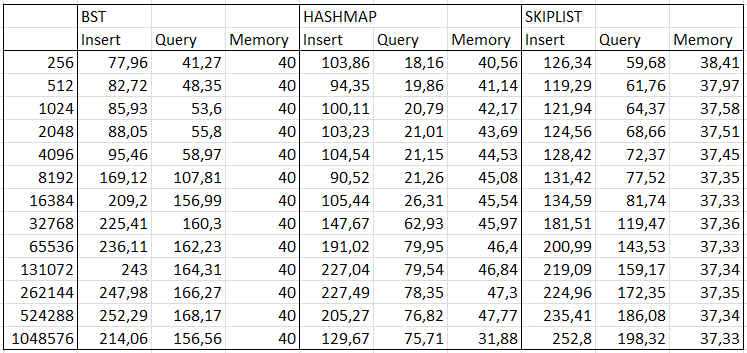
\includegraphics[width=\textwidth]{ip-address-averages.png}
    \caption{Per element averages with the IP-address key type.}
    \end{figure}

    \begin{figure}[h!]
    \centering
    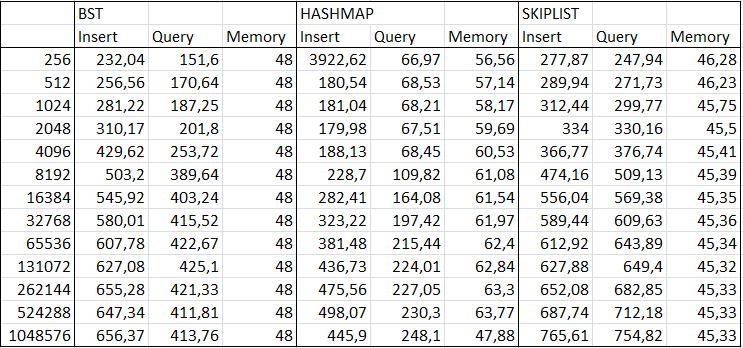
\includegraphics[width=\textwidth]{domain-averages.png}
    \caption{Per element averages with the domain key type.}
    \end{figure}

    \begin{figure}[h!]
    \centering
    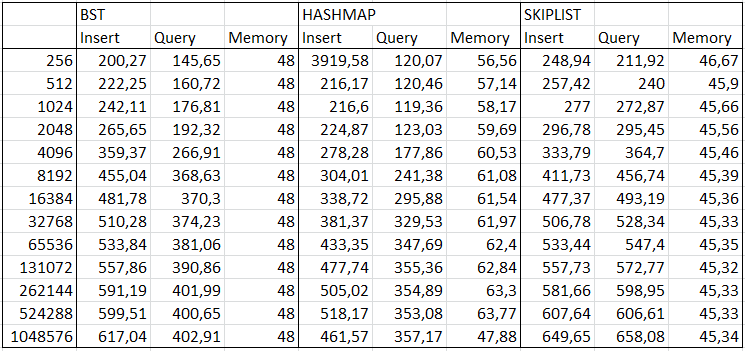
\includegraphics[width=\textwidth]{full-path-averages.png}
    \caption{Per element averages with the full path key type.}
    \end{figure}

\end{document}
